\documentclass[12pt]{article}

% PACKAGES

\usepackage[
top=2.50cm,
bottom=2.50cm,
left=2cm,
right=2cm,
marginparsep=0pt,
marginparwidth=0pt]{geometry}
\usepackage{fancyhdr}
\usepackage{float}
\usepackage{dirtree}
\usepackage{cancel}
\usepackage{mathtools}
\usepackage{amsmath}
\usepackage{amsthm}
\usepackage{amssymb}
\usepackage{textcomp}
\usepackage{ulem}
\usepackage{verbatim}
\usepackage{contour}
\usepackage{graphicx}
\usepackage{xcolor}
\usepackage[T1]{fontenc}
\usepackage{inputenc}
\usepackage[unicode]{hyperref}
\usepackage[shortlabels]{enumitem}
\usepackage{booktabs}
\usepackage{bookmark}
\usepackage{listings}
\usepackage{xcolor}
\usepackage{tocloft}
\usepackage{tikz}
\usepackage{subfiles}

% MACROS & DEFS

\newcommand{\floor}[1]{\left\lfloor #1 \right\rfloor}
\newcommand{\ceil}[1]{\left\lceil #1 \right\rceil}
\newcommand{\round}[1]{\left\lfloor #1 \right\rceil}
\newcommand{\abs}[1]{\left\lvert #1 \right\rvert}

\DeclareRobustCommand{\ul}[1]{%
	\uline{\phantom{#1}}%
	\llap{\contour{white}{#1}}%
}

\renewcommand{\ULdepth}{1.8pt}
\contourlength{0.8pt}

\setlength{\parindent}{0em}
\setlength{\parskip}{0.75em}

\definecolor{codegreen}{RGB}{0,135,0}
\definecolor{codegray}{RGB}{135,135,135}
\definecolor{codemagenta}{RGB}{215,0,135}
\definecolor{codepurple}{RGB}{135,0,175}
\definecolor{backcolour}{RGB}{238,238,238}

\def\cpp{{C\nolinebreak[4]\hspace{-.05em}\raisebox{.4ex}{\tiny\bf ++}}}

% PACKAGE CONFIG

% \graphicspath{ {./images/} }

\lstdefinestyle{code}{
	basicstyle=\ttfamily\small,
	commentstyle=\color{codegray}\itshape,
	keywordstyle=\color{codepurple},
	stringstyle=\color{codegreen},
	aboveskip=25pt,
    belowskip=10pt,
	breaklines=true,
	numbers=none,
	frame=tb,
	framesep=5pt,
	keepspaces=true,
	showspaces=false,
	showstringspaces=false,
	breakatwhitespace=false,
	tabsize=2,
	showtabs=false,
}

\lstset{style=code}

% Set dots for table of contents
\renewcommand{\cftdot}{.}
\renewcommand{\cftsecleader}{\cftdotfill{\cftdotsep}}

% Set theorem
\newtheorem*{definition}{Definition}

% HEADER & FOOTER

\setlength{\headheight}{15pt}
\pagestyle{fancy}
\renewcommand{\headrulewidth}{0pt}
\lhead{J. Scerri}
\chead{CPS2004 --- Assignment}
\rhead{\thepage}

% TITLE

\title{CPS2004 --- Object Oriented Programming\\
\vspace{1em}\textbf{Assignment}}

\date{\today}

\author {{\textbf{Juan Scerri}}\\
B.Sc. (Hons)(Melit.) Computing Science and Mathematics (Second Year)}

\begin{document}

%----------------------------------
%	TITLE PAGE
%----------------------------------

\maketitle % Print the title page

\thispagestyle{empty} % Suppress headers and footers on the title page

%----------------------------------

\tableofcontents

\clearpage

\listoffigures

\lstlistoflistings

\clearpage

\section{Plagiarism Declaration}

Plagiarism is defined as \textit{``the unacknowledged use, as
one's own, of work of another person, whether or not such work
has been published, and as may be further elaborated in Faculty
or University guidelines''} (\ul{University Assessment
Regulations}, 2009, Regulation 39 (b)(i), University of Malta).

I, the undersigned, declare that the report submitted is my
work, except where acknowledged and referenced. I understand
that the penalties for committing a breach of the regulations
include loss of marks; cancellation of examination results;
enforced suspension of studies; or expulsion from the degree
programme.

Work submitted without this signed declaration will not be
corrected, and will be given zero marks.

\vfill

\begin{minipage}[t]{0.3\textwidth}
\ul{Juan Scerri} \medskip

\textbf{Student's full name} \medskip
\end{minipage}
\hfill
\begin{minipage}[t]{0.3\textwidth}
\ul{CPS2004} \medskip

\textbf{Study-unit code} \medskip
\end{minipage}
\hfill
\begin{minipage}[t]{0.3\textwidth}
\ul{{\today}} \medskip

\textbf{Date of submission} \medskip
\end{minipage}

\vspace{2cm}

\textbf{Title of submitted work:} \ul{Object Oriented
Programming Assignment}

\vspace{2cm}

\textbf{Student's signature} \medskip

\underline{
\includegraphics[height=2cm]{./images/sig.png}} \medskip

% Specifically:
% - explain language choice 
% - explain the user interface and how to interact with the game
% - mention the design (with uml) and design choices
% - important technical aspects which are crucial and
%   fundamental to the whole program
% - approach to testing and ensuring proper functionality of the
%   program
% - limitations and possible improvements

\section{Village War Game}

\subsection{Language Choice}

Java was chosen for the Village War Game because it has more
complicated entity lifetimes. Programming the game in \cpp{}
would have required dealing with pointers to manage lifetimes.
Obviously, dealing with pointers brings the possibility of
memory leaks. Since Java has a Garbage Collector (GC) there is
no need for manual deallocation of memory.

\subsection{User Guide}

\subsubsection{Download, Compiling \& Running}

\begin{enumerate}
\item
    Clone the repository.
\begin{lstlisting}
$ git clone https://github.com/JuanScerriE/village-war-game
\end{lstlisting}

\item
    Compile the game.
\begin{lstlisting}
$ cd village-war-game ; ./compile.sh
\end{lstlisting}

\item
    Run the game.
\begin{lstlisting}
village-war-game $ ./run.sh
\end{lstlisting}

\end{enumerate}

\subsubsection{Playing}

% add image of specifying human players

Starting the game the player is asked to input the number of
human players.

% add image of specifying AI players

Then the player is aksed to input the number of AI players.

% add image of the menu

The game loop will start. Each human player will be prompted
with a menu of options. There are two categories: Info and
Actions. The Info category contains options which provide the
player with information about his own village, enemy villages,
armies and costs. The Actions category contains options which
affect the state of the game such as building, training and
attacking. Finally, the player can decided to pass the turn to
the next player.

Each player by default at the start will have 50 food, metal and
mana. The player can then use these resource to build or upgrade
buildings and train troops.

The following types of building can be built:

\begin{enumerate}
    \item Academy (to generate wizards)
    \item Foundation (to generate scouts)
    \item Arena (to generate brawlers)
    \item Farm (to generate food)
    \item Mine (to generate metal)
    \item Mana Tower (to generate mana)
\end{enumerate}

As described in the above list there are three types of troops:

\begin{enumerate}
    \item Wizard (high attack, low health, medium speed, low
        carrying capacity)
    \item Brawler (high attack, high health, slow speed, medium
        carrying capacity)
    \item Scout (low attack, medium health, high speed, high
        carrying capacity)
\end{enumerate}

\subsection{Design}
\subsection{Technical Aspects}
\subsection{Testing}
\subsection{Limitations \& Improvements}

\section{Minesweeper}

\subsection{Language Choice}

\cpp{} was chosen for Minesweeper because it has a fixed board
size of $16 \times 16$. This means that it is possible to stack
allocate every object removing the need for dynamic memory
allocation. This is facilitated by \texttt{std::array} from the
Standard Template Library (STL) which allows for the creation of
fixed size arrays on the stack.

\subsection{User Guide}

\subsubsection{Download, Compiling \& Running}

\begin{enumerate}
\item
    Clone the repository.
\begin{lstlisting}
$ git clone https://github.com/JuanScerriE/minesweeper
\end{lstlisting}

\item
    Compile the tests and the game.

    \textbf{Note:} Make sure that \texttt{gtest} and
    \texttt{ncurses} are installed for the tests and the game,
    respectively.
\begin{lstlisting}
$ cd minesweeper ; ./compile.sh
\end{lstlisting}

\item
    Run the tests.

    \textbf{Note:} Some tests might fail. This is because the
    implentation of \texttt{srand} and \texttt{rand} differ
    between platforms (specifically macOS and Linux).
\begin{lstlisting}
minesweeper $ ./tests.sh
\end{lstlisting}

\item
    Run the game.
\begin{lstlisting}
minesweeper $ ./run.sh
\end{lstlisting}

\end{enumerate}

\subsubsection{Playing}

\begin{figure}[H]
    \centering
    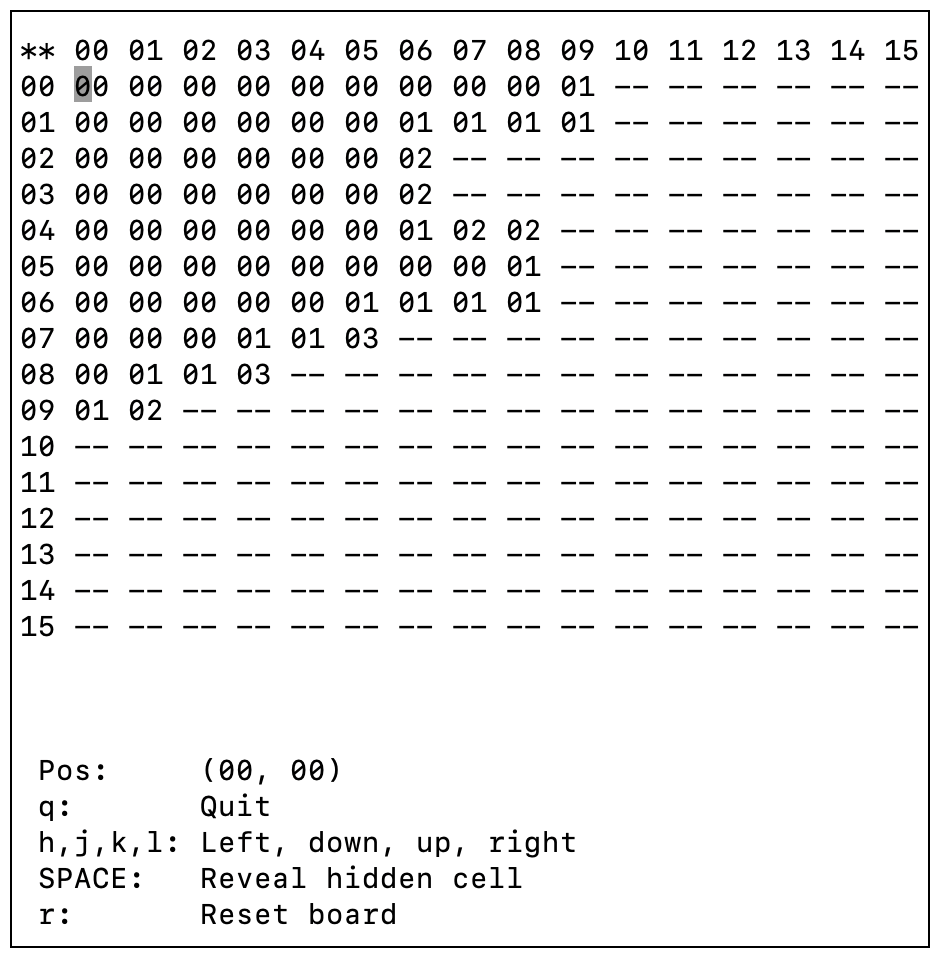
\includegraphics[width=10cm]{./images/playing-minesweeper.png}
    \caption{Playing Minesweeper}
    \label{playing-minesweeper}
\end{figure}

The general guide to playing Minesweeper is described above in
figure \ref{playing-minesweeper}.

\textbf{Note:} \texttt{vim} motions are used to move the cursor.

\begin{figure}[H]
    \centering
    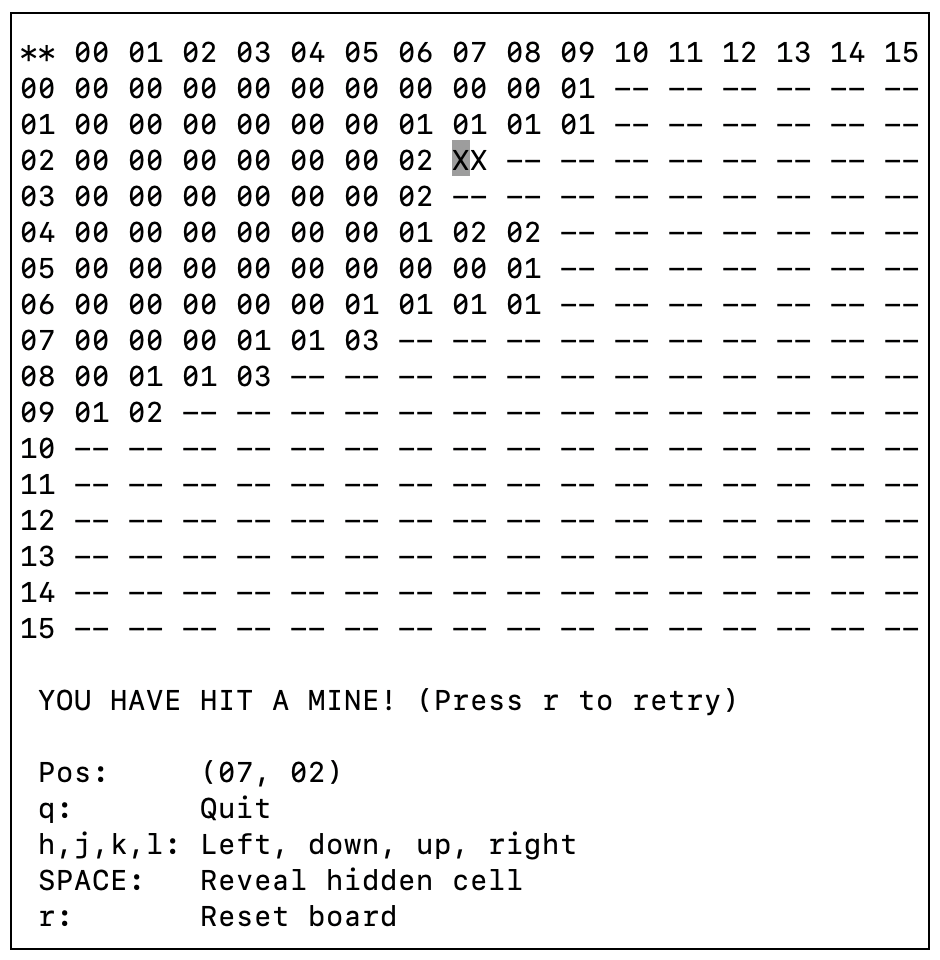
\includegraphics[width=10cm]{./images/hitting-mine-minesweeper.png}
    \caption{Hitting a mine}
    \label{hitting-mine-minesweeper}
\end{figure}

If the player hits a mine the above message as in figure
\ref{hitting-mine-minesweeper} will be displayed.

\begin{figure}[H]
    \centering
    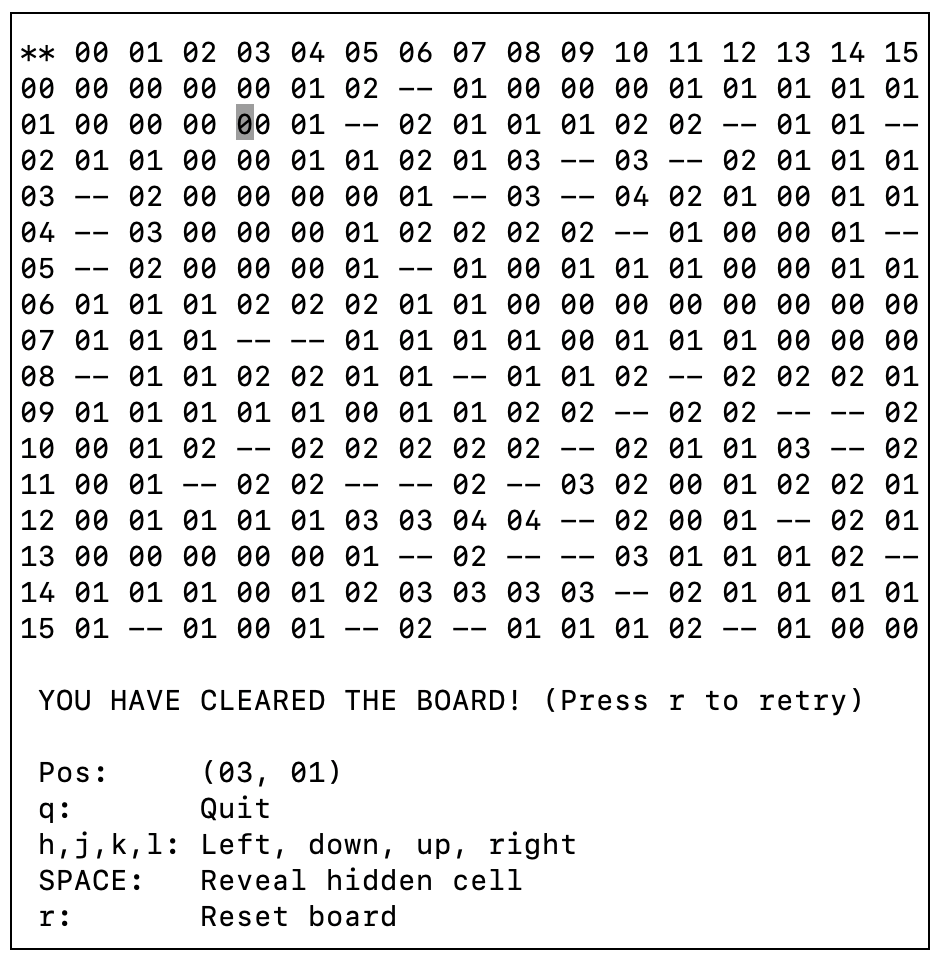
\includegraphics[width=10cm]{./images/finishing-minesweeper.png}
    \caption{Finishing a game of Minesweeper}
    \label{finishing-minesweeper}
\end{figure}

If the player manages to clear all the cells without hitting a
mine the above message as in figure \ref{finishing-minesweeper}
will be displayed.

Finally, there is an additional \textit{secret} command to
automatically complete the board without hitting a mine. The
user needs to press \texttt{W} (\texttt{shift + w}).

\textbf{Note:} This only works if the user has at least revealed
one cell. This is because the board is populated with all the
mines after the first reveal to ensure a player never hits a
mine on his first try.

\subsection{Design}

\begin{center}
\subfile{minesweeper-uml/minesweeper.latex}
\end{center}

\begin{center}
\subfile{minesweeper-uml/board.latex}
\end{center}

\begin{center}
\subfile{minesweeper-uml/cell.latex}
\end{center}

\begin{center}
\subfile{minesweeper-uml/relations.latex}
\end{center}

The Minesweeper class contains the user interface code, that
is it contains all \texttt{ncurses} specific code. The class
also handles user input.

The Board class contains the majority of the game logic. It is a
part of the Minesweeper class, that is if a Minesweeper object
ceases to exist so does the Board object. Further more the
actual board \texttt{m\_board} is a grid of Cell objects. Also
the lifetime of the objects is managed by the Board since when
the board ceases to exist so do the cells.

\subsection{Testing}

\begin{figure}[H]
    \centering
    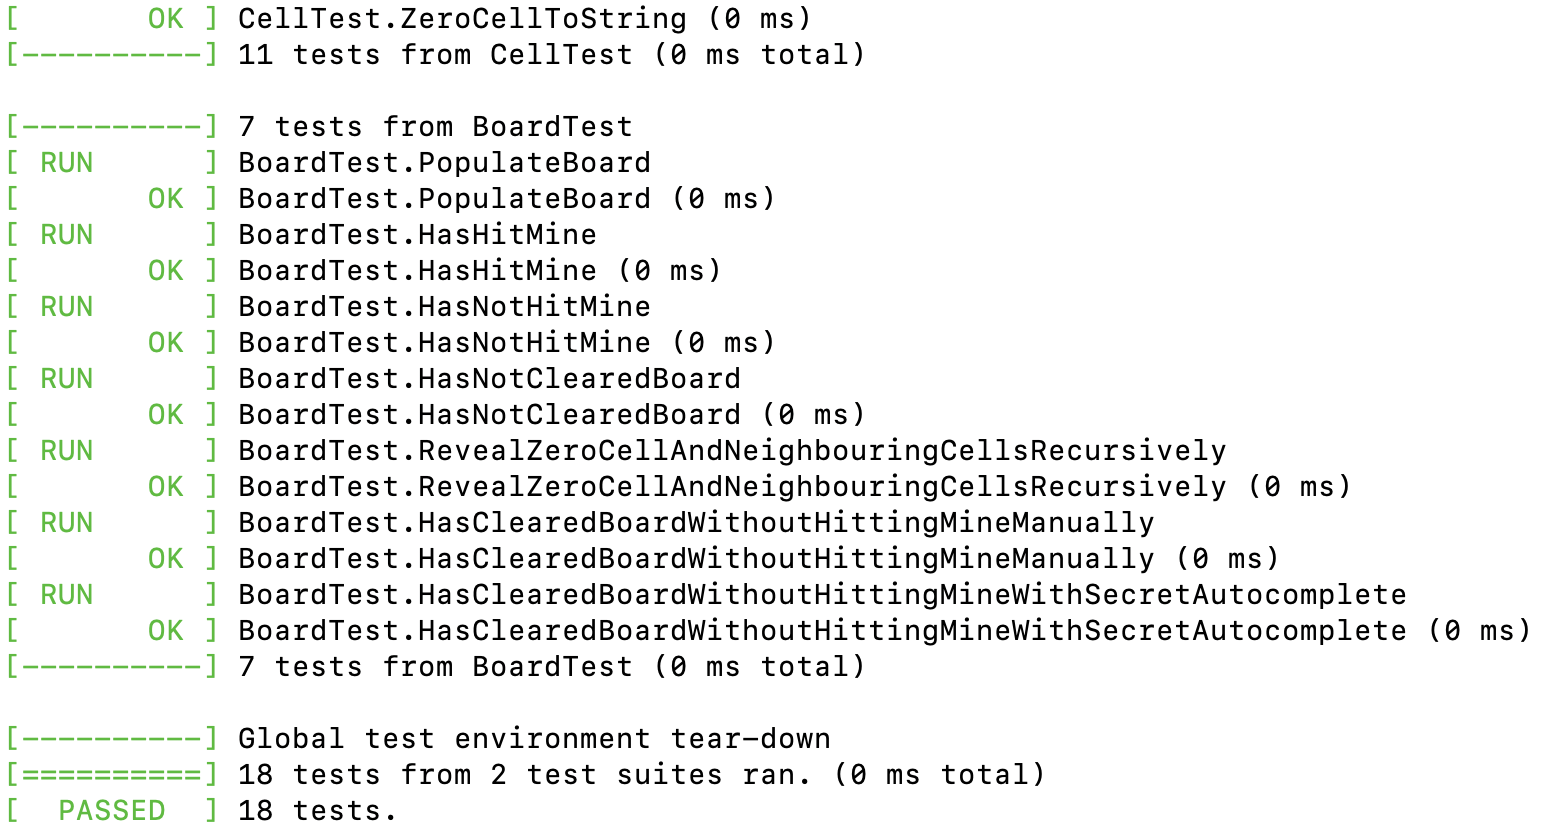
\includegraphics[width=10cm]{./images/unit-tests-minesweeper.png}
    \caption{Unit tests for Minesweeper (on macOS Ventura 13.1)}
\end{figure}

Black-box Testing and Unit Testing were used to test the
application. For unit testing \texttt{gtest} is required.

\begin{figure}[H]
    \centering
    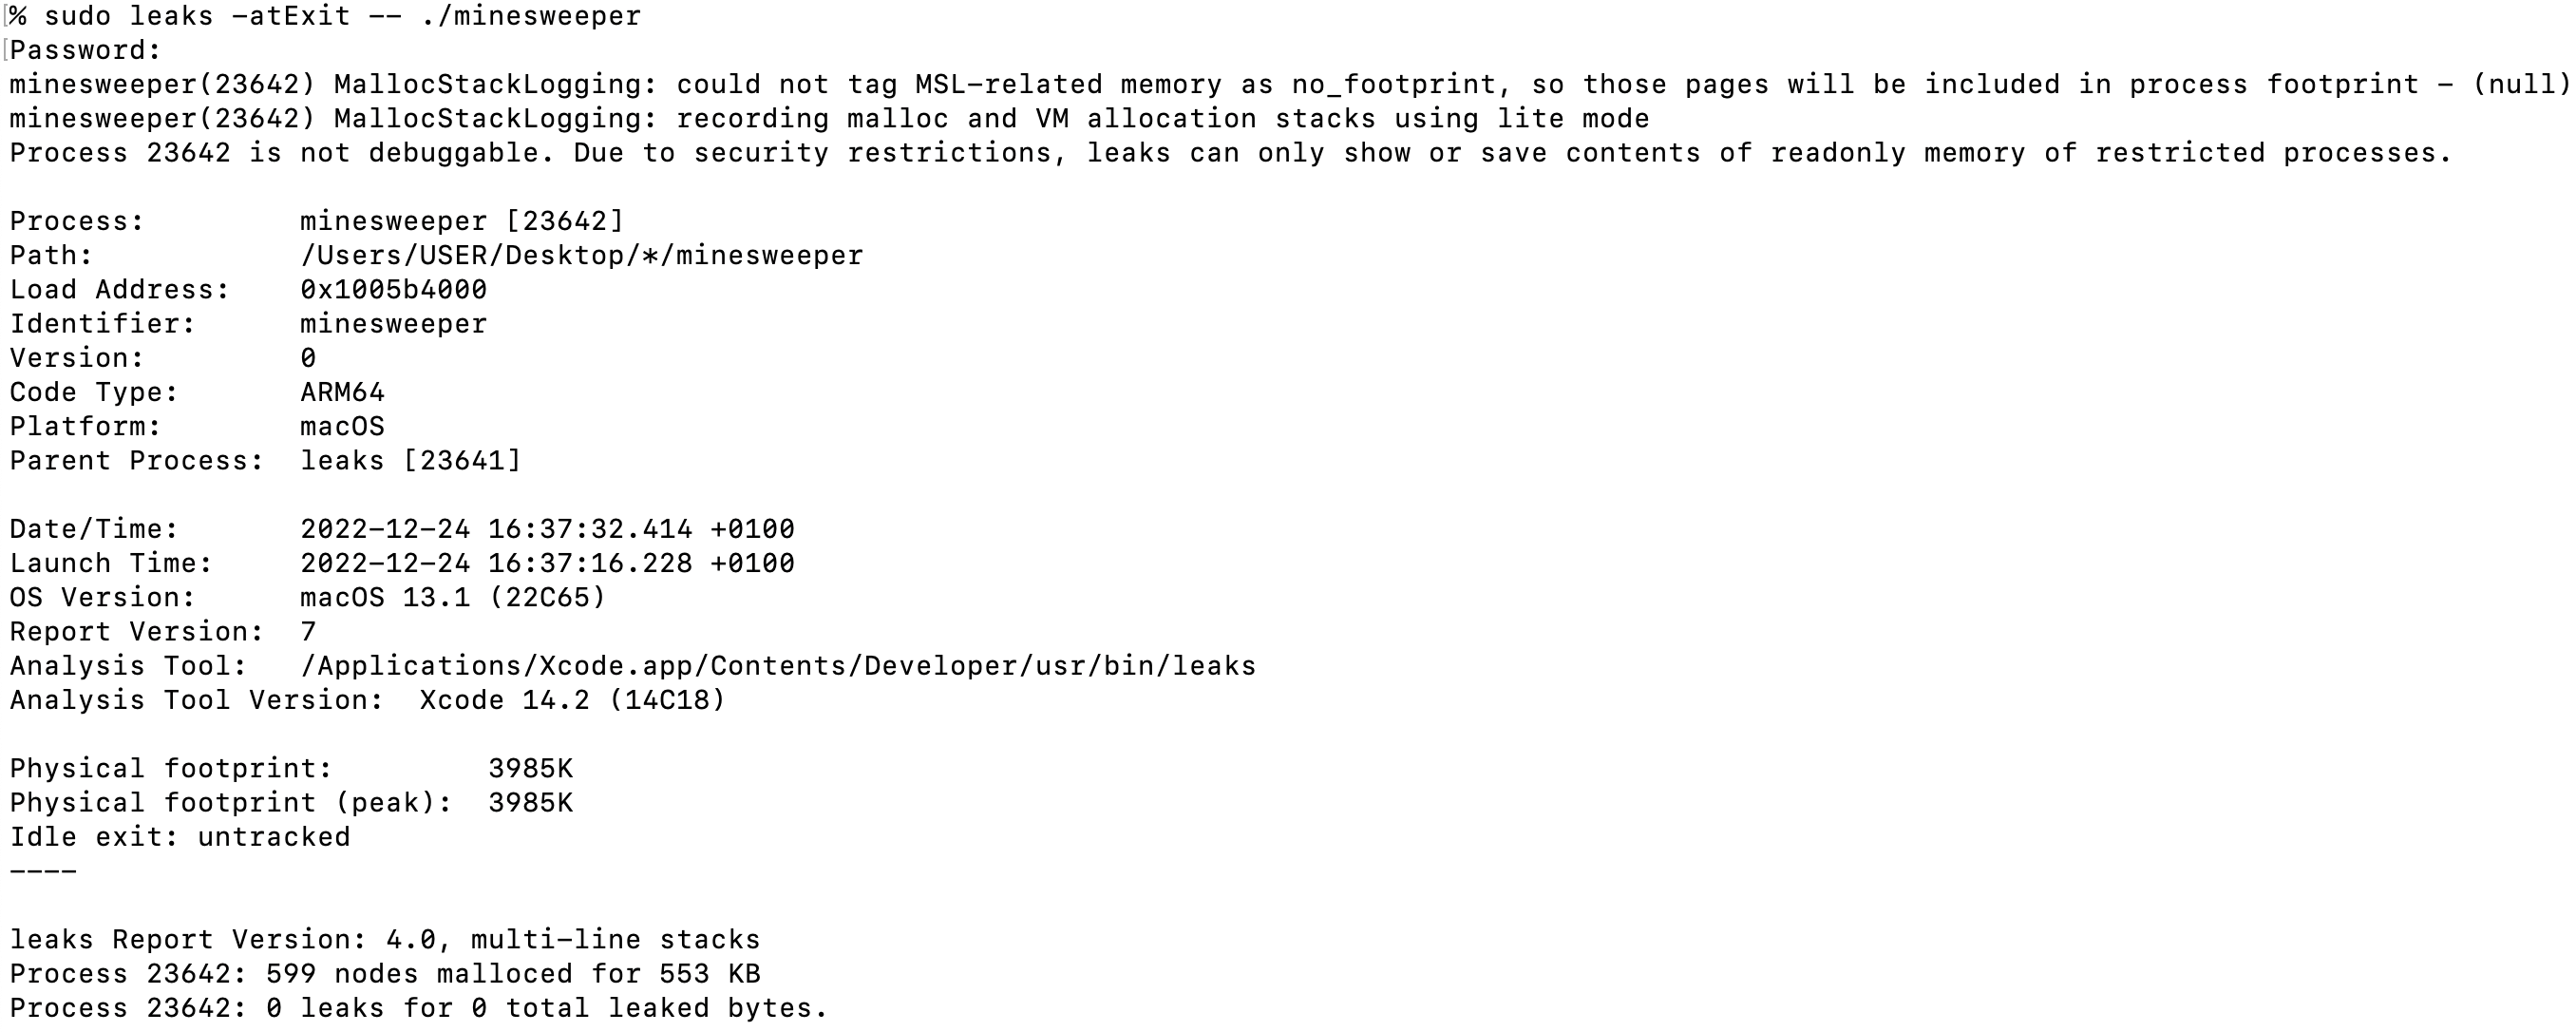
\includegraphics[width=14cm]{./images/leaks-minesweeper.png}
    \caption{Testing for memory leaks (on macOS Ventura 13.1)}
\end{figure}

Furthermore, to test for memory leaks, on macOS, \texttt{leaks}
was used and, on Linux, \texttt{valgrind} was used.
\texttt{leaks} reported not memory leaks whilst
\texttt{valgrind} reported leaks from \texttt{ncureses}.

\subsection{Limitations \& Improvements}

\ul{Limitation:} The unit tests are not cross-platform; four of
the unit tests fail on Linux. This is mostly due to differing
implementations of \texttt{srand()} and \texttt{rand()} on
different platforms.

\ul{Solution:} Create a custom random number generated. This
guarantees the same result across different platforms.

\ul{Limitation:} The \texttt{ncurses} library leaks memory on
Linux whilst on macOS it does not.

\ul{Solution:} This seems to be intended behaviour from
\texttt{ncurses}. Read the man page at
\url{https://man7.org/linux/man-pages/man3/curs_memleaks.3x.html}

\end{document}
